\documentclass[11pt]{article}
\usepackage[utf8]{inputenc}
\usepackage{setspace}
\usepackage{lineno}
\usepackage{authblk}
\usepackage{natbib}
\usepackage[margin=2cm]{geometry}
\usepackage{tabularx}
\newcommand{\supersc}[1]{\ensuremath{^{\textrm{#1}}}}
\newcommand{\subsc}[1]{\ensuremath{_{\textrm{#1}}}}
\usepackage{booktabs}
\bibliographystyle{unsrtnat}
\usepackage{pdfpages}

\title{%
	\textbf{Estimating movement patterns from camera trap data} \\
	\large MRes CMEE project proposal}
\author[1]{Lizzie Bru}
\affil[1]{School of Life Sciences, Imperial College London, Silwood Park Campus, Ascot SL5 7PY, UK}
\date{December 2021}

\onehalfspacing
\linenumbers

\begin{document}
	
	\maketitle
	
	\begin{center}
		Primary external supervisor: Dr Marcus Rowcliffe (Zoological Society of London)
	\end{center}

	\begin{center}
		Primary internal supervisor: Dr James Rosindell (Imperial College London)
	\end{center}

	\begin{center}
		Secondary external supervisor: Dr Chris Carbone (Zoological Society of London)
	\end{center}
	
	\begin{center}
		Secondary internal supervisor: Francis Windram (Imperial College London)
	\end{center}
	


	
	\newpage
	
	\section{Background and motivation}
	
	Understanding movement patterns of animals in the wild is important in behavioural and ecological research. Estimating movement speed is particularly interesting and important as it informs us on both short and long temporal scales. In the short-term, speed can reflect bouts of activity and affects phenomena such as rates of resource and predator encounters and of energy expenditure (\cite{schmidt1972locomotion, pyke1981optimal}). Over longer temporal scales, measures of speed can indicate space use. Hence estimating animals' speeds of movement can inform us on individual behaviours notably involving predation risk, dietary habits, and energy constraints (\textit{e.g.,} \cite{miller2014amur}), as well as population-level behaviours including population processes (\textit{e.g.,} \cite{werner1993ecological}) and human-wildlife interactions (\textit{e.g.,} \cite{graham2009movement}).
	
	Camera trap data has the potential to substantially aid research of animal movement patterns. While telemetry is commonly used to study movement patterns in the wild, it is invasive and limited in scope to only a few tagged individuals. Furthermore, studies measuring speed using telemetry are often in practice based on telemetry data where distances measured are of low resolution due to low frequency of fixes (\cite{rowcliffe2012bias}). Camera traps can overcome many of these limitations, providing a valuable alternative to GPS tracking. Camera trapping is non-invasive, can provide information about a greater number of individuals, and can provide data with high temporal resolution (with fixes at least every second for video or near-video rapid-fire settings).
	
	While some studies have so far used camera trap data to estimate movement patterns, there is scope for improvement. In particular, \cite{rowcliffe2016wildlife} describe and validate a new approach for estimating speed from camera trap data. When estimating mean speed from estimates of speed derived from simple relationships between speed, distance, and time, they use maximum likelihood to take into account the fact that the observed distribution of speeds is likely size-biased (\cite{patil2006weighted}); animals are more likely to be caught on camera traps when moving faster. They therefore fit size-biased probability distributions to a sample of speed observations to estimate average speed of travel. However, their method involves assuming that there is a linear relationship between speed and trap rate, based on the random encounter model equation described in \cite{rowcliffe2008estimating}. This assumption has not been empirically tested and may not be fair to make. It may indeed often be wrong especially for species with dichotomous movement patterns. Their method also may be biased by camera traps being more likely to 'miss' the final steps of fast movements made up of long step-lengths. Later work from \cite{palencia2021innovations} has sought to improve \cite{rowcliffe2016wildlife}'s method, although the robustness of their method may remain in doubt.
	
	In this project I will therefore aim to develop a better method of estimating speed from camera trap data.
	
	\newpage
	\section{Proposed work}
	
	\subsection{Part I: Theoretical component: the movement ecology of mammals}
	
	Initially, I will investigate generally how behaviour interacts with camera trap data. In particular, I hope to examine how and how well camera trap data enable us to capture behavioural shifts between different movement states, and more generally hence enable the study of the behavioural ecology of foraging patterns. I would also like to investigate how contacts and encounters can be captured using camera trap data, notably regarding delineating the interval between fixes of different individuals at which they are considered contacts, and looking for autocorrelations in contacts. It would also be interesting to investigate how scaling may affect all of the above, using data on mammals ranging in size from mice to deer. 
	I hope to then use my findings in this first step to address how they influence issues we have with camera trap estimates.
	
	
	\subsection{Part II: Methodological component: estimating movement patterns from camera trap data}
	
	The principle element of this project will be to investigate how to improve methods used to estimate speed from camera trap data. Most of the work will involve using simulations.
	
	\subsubsection{How to measure speed}
	
	I will firstly address whether initial measures of speed from camera trap data can be improved upon. To do this, I will primarily build on work from \cite{rowcliffe2016wildlife}. A potential approach involves using simulated random walks to program exact movement speeds and assessing the results of various approaches for calculating average speed against simulations.
	
	\subsubsection{How to post-adjust speed estimates to take biases into account}
	
	I will then examine how speed estimates can be post-adjusted to take two principle biases into account.
	
	Firstly, a potential positive bias is that animal speed may be proportional to trap rate. As part of this, I may additionally include consideration of the technical aspects of camera traps, specifically how their physical properties may lead them to tend to miss more high-speed movements.
	
	Secondly, a potential negative bias is that camera traps may be more likely to miss the final big step lengths of animals moving at faster speeds and with longer step-lengths. 
	
	Building on from this, if I am able to identify sources of bias, it would be interesting to then investigate which species are mostly likely to be associated with such biases and hence for whom speed estimates may be most unreliable.
	
	\subsection{Part III: Ecological component: demonstrating the utility of this method}
	
	I would then like to give this project some ecological grounding by conducting a proof-of-concept for any methods which I come up with in Part II. This would be used to demonstrate that my methods work and that they can be useful in behavioural and ecological research, particularly in a conservation setting. I could for instance do so by using my methods to answer ecological questions such as whether variables, for example urbanisation, predict animal movement speed.
	
	
	\subsection{Data}
	
	For this project I will use camera trap data provided by the Zoological Society of London (ZSL). They currently have tagged data collected in London containing around ten different mammal species ranging from mice to deer, as well as bird data although I am less likely to use this since estimating speed of bird movement is more complicated due to additional dimensionality. These data also contain estimates of tracks of each animals' movement and some contact data as well. One potential caveat which I intend to address is that these data are predominantly collected between 5pm and 9am, so this could bias my work. However, I do not anticipate this being deeply problematic.
	
		
	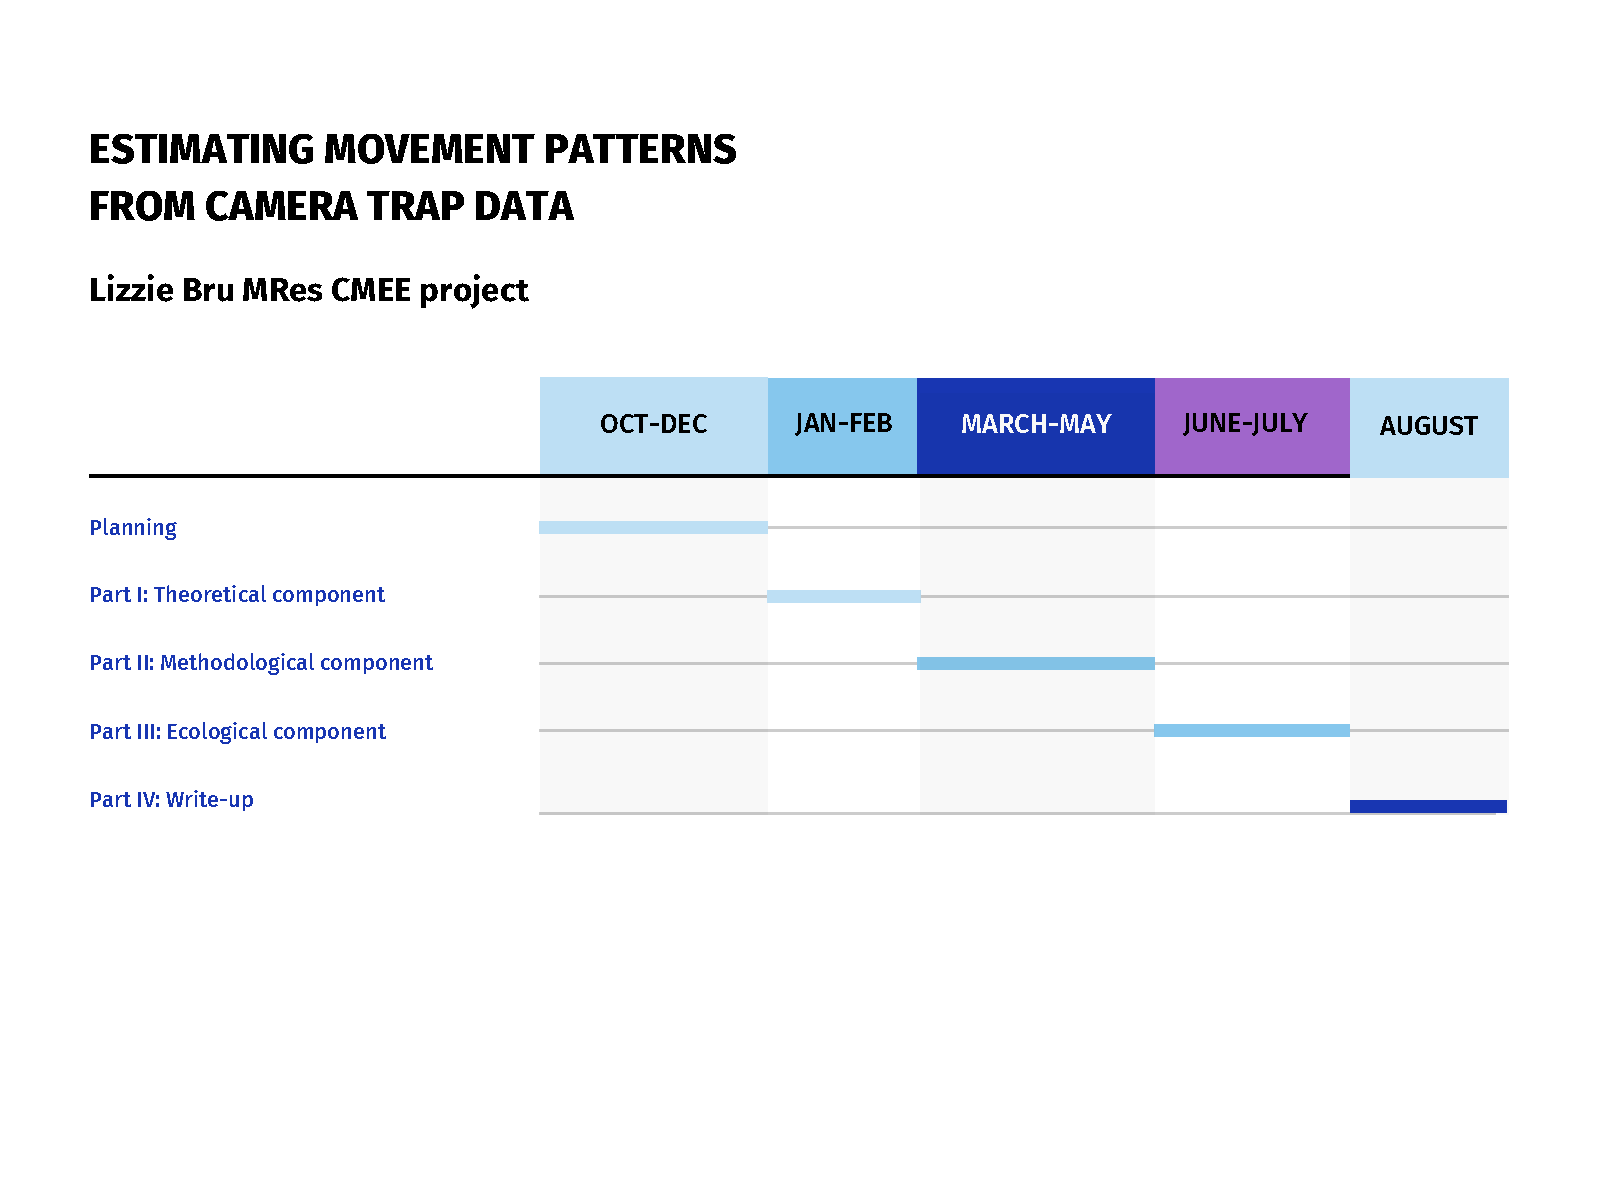
\includepdf[pagecommand=\section{Gantt chart}]{ganttchart.pdf}

	
	
	\bibliography{proposalbiblio.bib}
	
\end{document}